\chapter{Music learning applications in AR}

\section{Introduction}

The DVIC augmented mirror overlays various digital information on top of the natural reflection of the user's head and upper body. Such overlaid information can be useful for the learning of embodied skills, and applications have already been created for the mirror to help people learn sign language and dance.

Currently the most common way to learn singing is through: 
\begin{itemize}
    \item Recording and listening to one’s own performances. 
    \item Taking a good posture, which is important to learn to sing in tune.
    \item Paying attention to one’s breathing, which is the basis of vocal technique and can be improved through breathing exercises.
    \item Performing vocalization exercises, which require a lot of patience.
    \item A capella singing, practised by listening to and learning a piece many times before reinterpreting it. 
\end{itemize}
   

This project explores how the mirror can help people learn music, and in particular, singing. Seeing one's reflection is useful when practicing singing because it allows the monitoring of one's posture. The mirror adds the ability to monitor one's pitch accuracy. This is done by adding a frequency tracking module that estimates notes sung by the user and an interface that gives the user real-time visual feedback.
The user can then train his or her ability to sing in tune by comparing the target frequency with that actually sung. This ability is called musical imagery, the ability to "imaginate" a note before playing/singing it \cite{godoy2012musical}. It can be perfected with practice. This ability is very important for a musician as it allows him/her to visualise a gap between two notes he/she wants to play/sing, and to translate it on his/her instrument or by voice.

Practicing music can be very laborious, long, and difficult. For example, practicing singing requires attending singing classes that teach you to visualize the right note in your head before you sing it. Singing also requires good posture and breath control to be effective.
The interactive mirror has the potential to give users the ability to monitor their posture, an important element in singing. The user can get double feedback by singing in front of the augmented mirror. He can see the position of the notes in relation to the ones he is singing and can correct himself.
At the same time, he sees his reflection in the mirror and can correct his posture to sing more effectively. In order to implement the singing application, a frequency tracking module estimates the notes sung by the user, and the user interface gives feedback on the accuracy of his pitch.
The singer can also activate a tutorial with falling notes, activate the playback of music to learn it before singing it, and use a calibration to set the singable range of notes for him.

\section{Related work}

\subsection{Singing Learning Applications}

The development of new electronic musical interfaces gives rise to potential novel approaches in music education. The gestual interactive systems and interfaces have great potential for practice in music pedagogy \cite{farrugia2015tunes}.
A number of smartphone apps exist for people learning to sing that focus on giving feedback on correct intonation.
Yousician is a fairly comprehensive application that allows you to quickly learn and master piano, guitar, bass, singing, and other instruments by practicing on your real instrument.
It offers to learn music theory through special exercises and lessons. The application listens to the user singing/playing, evaluates his/her performance with a frequency estimation, and proposes to play different songs with tutorials and games. 

\begin{marginfigure}
    \centering
    \includegraphics{AdrLfv_master_thesis/images/yousician.png}
    \caption{Yousician interface.}
    \label{fig:yousician}
\end{marginfigure}

It offers a system of notes in the form of bars coming from the right, which the user must sing afterwards (see figure \ref{fig:yousician}). If he sings right, the bar turns green, if not, red.

Other applications are very similar such as Sing Sharp, LearnSing... Riyaz is another application that allows you to load existing music to generate the notes of the song, and then view a tutorial of these falling notes.
The application then gives statistics on the performance: pitch accuracy, control and breathing capacity, vocal range. These applications often start by determining a range of frequencies that the person can perform with the voice before starting the singing training. This allows the tutorial to be tailored to the user’s vocal abilities.

The general strategy of these applications is to use learning methods by practice, measurement, and correction. The classic operation is the realization of tutorials on the placement of the hands for an instrument, or the position of the notes to be sung for the note, then by a graphic feedback with the visualization of the fact that a note has been correctly sung or not.
It is possible to learn how to play music by means of video games created for this purpose. Among the best known video games in this field are Guitar Hero and Rock Band. These two games allow you to learn to play the guitar in a fun way, always using a system of falling notes \cite{farrugia2015tunes}.

\subsection{Music Practise}

\paragraph{Music practise assisted by AR}

Augmented reality, which involves the integration of virtual objects into the real world and enabling interactivity through sensor technology, presents a novel paradigm for practical applications.

\begin{marginfigure}
    \centering
    \includegraphics{AdrLfv_master_thesis/images/Wireless-sensor-interface.jpg}
    \caption{Teacher and student using the system during a music class \cite{bevilacqua2007wireless}.}
    \label{fig:Wireless-sensor-interface}
\end{marginfigure}

Frederic Bevilacqua \& al. proposed a project with miniature wireless sensor system that is used with accelerometers and gyroscopes to make gesture recognition in musical pedagocial scenarios (see figure \ref{fig:Wireless-sensor-interface}). Music teaching methods are often based on playful approaches and exercises focusing on body movements. The project aimed to experience and practice “smoothness” and “fluidity” of musical gestures by analizing the curves of the movements \cite{bevilacqua2007wireless}.

\begin{marginfigure}
    \centering
    \includegraphics{AdrLfv_master_thesis/images/Practice-Session.png}
    \caption{Practice Session Work Map of an expert player (E-1)’s hour-long practice of Chopin’s “Mazurka in A minor, Op. 17 No. 4".}
    \label{fig:Practice-Session}
\end{marginfigure}

Yu Ting Hang et al. proposed a visual interface for learning singing on the Internet. The aim is to link pitch and musical notation through frequency estimation and waveform recognition. The visualization of the sung notes in relation to the desired ones allows to correct vocal accuracy errors and thus to practice singing by sight \cite{huang2016visualized} (see figure \ref{fig:Practice-Session}).

In this context of music assisted with AR,Giovanni Santini \cite{santini_giovanni_2020_4813449} delve into sound processing and synthesis facilitated by sensors, thereby unveiling innovative avenues for musical experimentation. Their work sheds light on the promising prospects that augmented reality offers in the augmentation of musical instruments, emphasizing the pivotal role of interface design in shaping the musical experience.
The article highlights several notable projects at the intersection of augmented reality (AR) and musical instrument augmentation pertinent to our research endeavor. 

\begin{marginfigure}
    \centering
    \includegraphics{AdrLfv_master_thesis/images/chromachord.png}
    \caption{Performer operating ChromaChord. Oculus Rift and Leap Motion.}
    \label{fig:chromachord}
\end{marginfigure}

ChromaChord \cite{fillwalk2015chromachord} is another example standing out as an initiative enabling users to engage with virtual interfaces through motion capture devices like Leap Motion and Oculus Rift (see figure \ref{fig:chromachord}). In this setup, virtual objects produce sound upon interaction with the user's hands. The users can play music by interacting with virtual strings in a three-dimensional environment. ChromaChord has potential applications in music education, composition, live performance, art creation, and other areas of music and VR.

\begin{marginfigure}
    \centering
    \includegraphics{AdrLfv_master_thesis/images/vrmin.png}
    \caption{A student practicing the theremin using VRMin with capture of the view on the right.}
    \label{fig:vrmin}
\end{marginfigure}

VRMin \cite{johnson2017vrmin} is a virtual reality application that employs principles akin to AR interfaces to enhance the Theremin, thereby elevating gaming precision through virtual spatial representations \ref{fig:vrmin}. The project combines sensor input from the physical theremin with visual cues and feedback in a virtual environment to provide an enhanced learning experience. 

Pianolens is an augmented reality system offering a dynamic and interactive sheet music display interface. The program displays intricate musical elements through intuitive adaptations to the sheet music and imparts comprehensive guidance on mastering new compositions, including precise timing and fingering techniques. 

\begin{marginfigure}
    \centering
    \includegraphics{AdrLfv_master_thesis/images/PianoLens-demonstration.jpg}
    \caption{PianoLens demonstration.}
    \label{fig:pianolens}
\end{marginfigure}

The approach involves the utilization of colored blocks in an interactive musical setting. These blocks possess widths commensurate with the corresponding piano keys and lengths proportional to the note duration (see figure \ref{fig:pianolens}). They are set in motion towards the performer and intersect with a specific reference line, denoting the "current" moment. At this juncture, the pianist is required to depress the relevant piano key and sustain the keypress until the block's conclusion. Additionally, these systems offer real-time feedback regarding the accuracy of note execution and rhythmic precision.

The features accelerate the acquisition of novel musical pieces but also elevate learner engagement during the rehearsal phase, standing as an effective tool in the field of music education and performance.

These illustrative examples underscore the diversity of projects that unite music, AR, and instrumental augmentation, paving the way for fresh opportunities in interaction and musical expression. Each of these projects tackles the design of AR interfaces in distinctive ways, all aimed at enhancing musical practice.

\paragraph{Music practice assisted by frequency estimation}


Kin Wah Edward Lin et al. presented a self-learning tool for singing on the smartphone. It allows the user to improve timing and intonation in a similar way to the previous project. It uses an intonation level classifier, a user performance rating mechanism, and a pitch training tool. 

\begin{marginfigure}
    \centering
    \includegraphics{AdrLfv_master_thesis/images/Intonation-Level-Classifier.png}
    \caption{Intonation Level Classifier with Song - Fly Me to the Moon \cite{lin2014implementation}.}
    \label{fig:Intonation-Level-Classifier}
\end{marginfigure}

The mix of visual demonstration/feedback is natural to understand and useful (see figure \ref{fig:Intonation-Level-Classifier}). The user’s intonation score improved by an average of 94.81 \% after training.

Philip McLeod \cite{mcleodtartini} presents a program called "Tartini" developed by Philip McLeod of the University of Otago in New Zealand.Tartini is a program intended to provide real-time music analysis tools to musicians. It uses a microphone and computer to provide precise visual feedback on elements such as intonation, intensity and shape of vibrato.The project aims to help musicians improve their musical technique, focusing mainly on pitch-related aspects of music.

\section{Singing Learning Program in AR}

\subsection{Context}

The DVIC augmented mirror project aims to change the way we perform certain tasks and disciplines in everyday life.
It adds a dimension of interactivity through our reflection, our position, our movements.

The mirror’s 3D camera makes it possible to precisely estimate the position of the user in  space. The person can then interact remotely, without touching the screen. A Plexiglas screen positioned above the screen of the device reflects the reflection of the user. This allows the display of elements over a reflection and thus interact with elements in augmented reality. The mirror’s augmentation gives people more awareness of their position and their movements. It allows full-body interactions with digital information, rather than accessing it through the small screens of computers and mobile devices. The added value of the project is to exploit mainly kinesthesia (which is not possible with other more traditional devices) as well as other forms of interaction. This is in addition to the various ways of interacting with the human body (human inputs/outputs) that can be exploited by the electronic devices we use every day.

Applications allow for example to have a return of its position with the display of a mediapipe skeleton above its reflection, to learn elements of sign language thanks to a training module, as well as to test other games. One of the primary uses of the mirror is to enable much better learning, using as many forms of intelligence as possible.

\subsection{Overview}

The objective of the project is to be an example of a module allowing people to learn the practice of a musical instrument on the mirror. As the device only requires the person in front of it without any material, a musical module would not have been suitable for most musical instruments.

\begin{figure}[h]
    \centering
    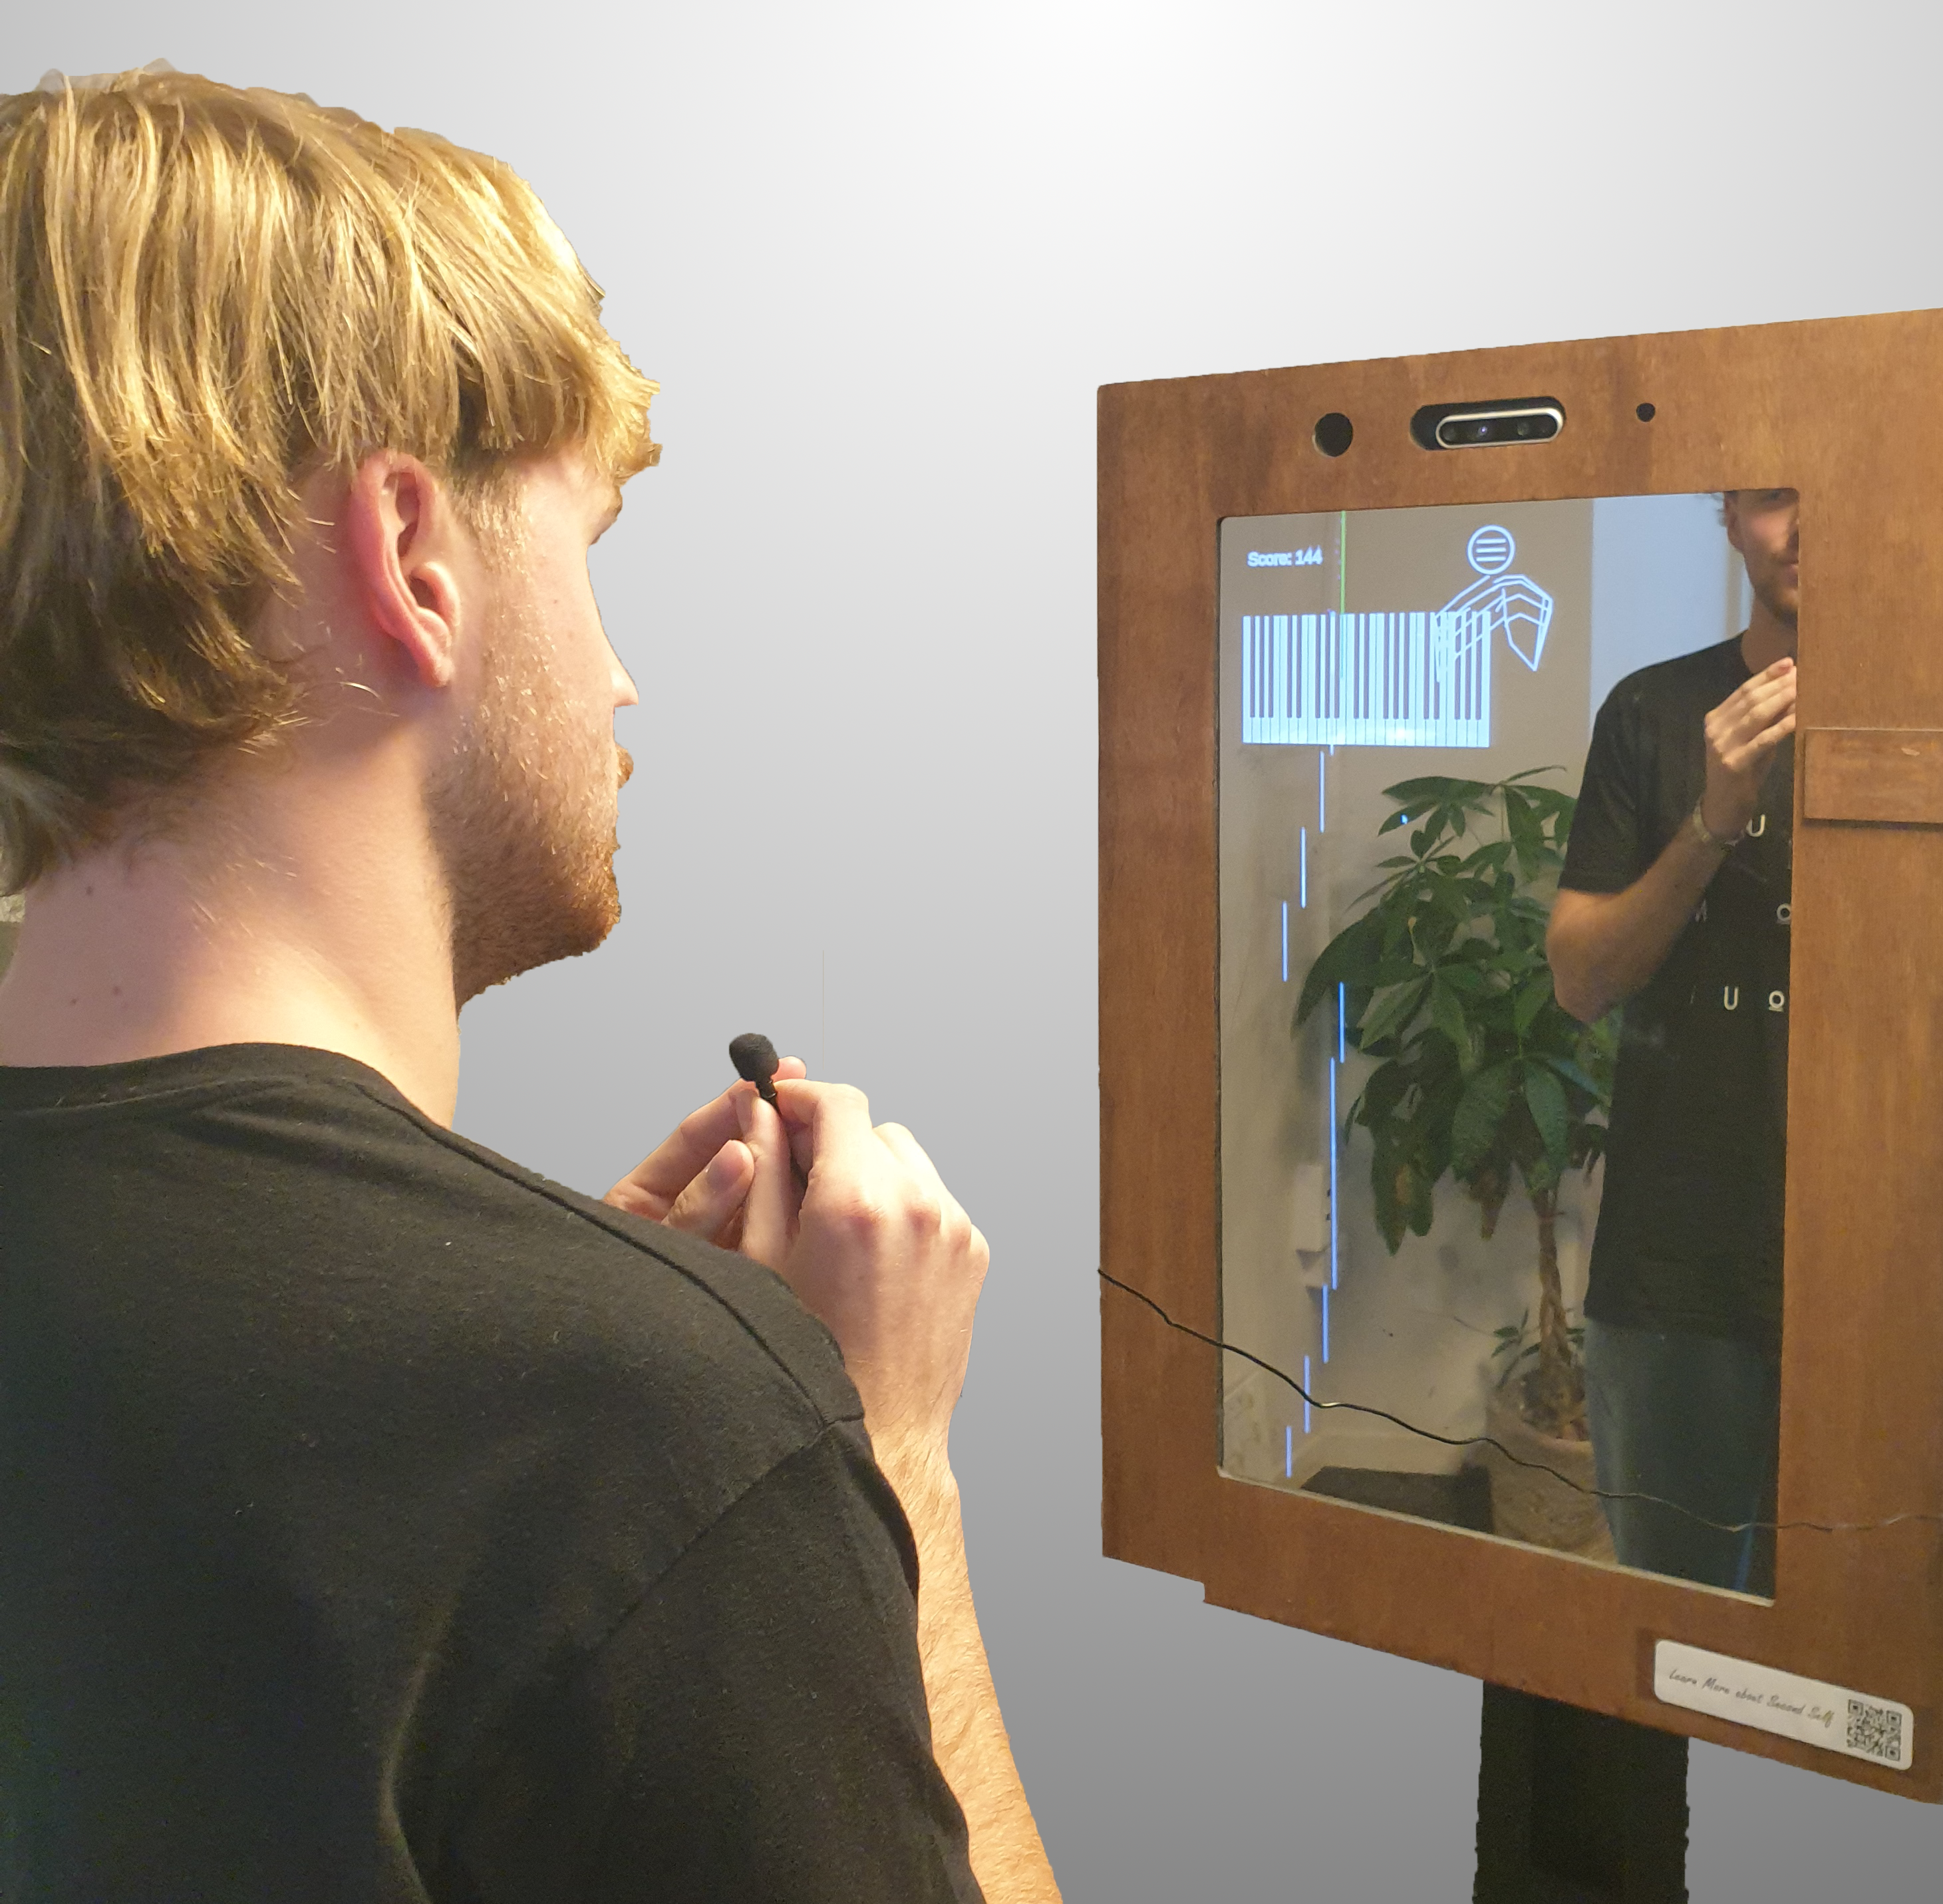
\includegraphics[width=2.2\columnwidth]{AdrLfv_master_thesis/images/cyprien_user_test.png}
    \caption{A user testing the musing training application.}
    \label{fig:cyprien_user_test.png}
\end{figure}

The project is based on frequency estimation for practice. A user plays an instrument or sings in front of the mirror (see figure \ref{fig:xiao_singing}). The mirror collects the frequency emitted and displays it on the screen.

The user sees the frequency he or she is emitting represented by a dot on the screen with a particle effect. The lower the frequency, the further to the left the dot is, and vice versa. Some options can be launched from the sub-menu of the "music\_training" application already
implemented on the mirror. The user can launch different music tutorials.

For example, he can launch the tutorial "La vie en rose", notes fall from the top of the screen and he must play them in rhythm. The module no longer has any aspect related to movement or position but only to the frequency emitted by the instrument or by the voice.
When the user sings correctly, the bars falling from the top change colour, gradually turning green and the particle effect on the dot intensifies (see figure \ref{fig:music_training}). They become increasingly red when the user sings out of tune. The score achieved is displayed for a few seconds at the end of the song.

\begin{figure}[h]
    \centering
    \includegraphics[width=2.2\columnwidth]{AdrLfv_master_thesis/images/music_training.png}
    \caption{The interface of the music learning application.}
    \label{fig:music_training}
\end{figure}

The vision of the project is to train the user to more or less consciously link the manipulation of the instrument or his voice with the sound he visualises in his head. The visual present on the mirror allows him to know where he is, if he has played/sung the right note and how to correct it if not.
This approach is different because it offers different options in the display. The user can launch different music tutorials, display bars to locate notes, erase them, as well as display the position of his hands.
Practising on a mirror is a plus as the user practices standing up unlike with a telephone. This makes it easier to practice singing because the body remains upright. This project is intended to be suitable for multiple instruments, while being entertaining and instructive.

\subsection{General Architecture}

The augmented mirror system runs on an operating system software called GOSAI. The music practice module takes the form of a JavaScript application coded directly on it. It uses the P5 library to display 2D elements and create the sketch. The backend uses two drivers coded on GOSAI: a new driver allowing the OS to use the microphone of the device and another driver allowing to make frequency estimation listening to the microphone. The latter takes a sound wave generated as an input and returns a musical frequency.

The GOSAI microphone driver takes the audio stream from the device hardware. It passes the data to the "frequency\_estimation" module which detects the frequency emitted in the audio stream as well as the gain and other parameters. This module places this data in the Reddis data. The processing.py file retrieves the frequency estimation data from the data and sends it to the display.js with socket.io. The display initializes a new music workout and sends it the necessary data to run.

New various tools such as the sub-menu system are coded on GOSAI for the project. The sub-menu allows the applications to propose options to be activated or deactivated manually by the user thanks to the estimation pose according to his desires.

\subsection{User Tests}

The user tests in this project aim to assess a user’s facilitation of learning to sing with the
mirror compared to other conventional tools.

\paragraph{Conduct of the user learning test}

We evaluate the difference between classical learning through "a capella" practice and learning with dynamic correction on the mirror. 

A randomly chosen user listens to the first few seconds of "La vie en rose - Carolina Eyck - theremin"  \cite{carolina_eyck_theremine} one time. He must then sing it in playback while listening to it in his headphones .
We record his singing performance to evaluate it later.

In a second part, he tests the application on the mirror. He then follows the 10 seconds tutorial with the falling notes. We record his singing performance to evaluate it later.

We realize these experiments in this order with 2 users each. We also conduct this experiment by reverting the order of experiments (first the program with music, and then the singing without visual support) with 2 other users.

\paragraph{Evaluation of the user experience}
\label{sec:eval_user_exp}

Here are the areas evaluated and the questions asked to the program testers. Their opinion is measured with a score out of 10 points.
Evaluation of the motivation to learn with this type of interaction: -Average motivation to learn this particular way. -Average fun in interacting.
Evaluation of the comprehensibility of the module: -Ease of understanding what needs to be done Evaluation of the estimation/display system: -Usability of the overall system, responsiveness, accuracy, smoothness of display. -Practicality of the design, position of the notes, graphics chosen for the different elements. The rendering estimated and displayed in the application should be smooth and not display any other spurious frequencies measured by the microphone. Problems of this kind can lead to the display of unsung frequencies as well as "skipping" of the cursor displaying the sung note. 

Evaluation of the tutorial method with falling notes. -Relevance and effectiveness of the tutorial method with falling notes rather than another.
Evaluation of the use of the reflection. -Does the use of the reflection in the glass seem to be a good potential for improving one’s vocal practice. Finally, the subject is asked about their remarks, suggestions and other constructive comments about the project.

\subsection{Results}

After testing four users singing the same music in playback, we observed a total number of errors of 6 imprecise semitones out of the 20 notes sung. We observe an inconsistent rhythm with successive accelerations and slowdowns. From the middle of the piece (containing the most complicated parts to reproduce), the number of errors increases considerably.

Users singing with the program achieved a score of 5 inaccurate semitones out of the 20 notes of the song. We observe a much better consistency of rhythm with little shift for each note. The user generally corrects the slight shift in the rhythm from one note to the following. During the two tests, we observed most errors during the large grade intervals (E3 to C3, then C3 to B3).

Users of the program gave an average rating of 6/10 for fun with the device, a rating of 8/10 for ease of understanding what needs to be done, a rating of 7/10 for accuracy and responsiveness of the program, a score of 7/10 in the practicality of the user interface and a score of 9/10 in the relevance of a falling notes tutorial for singing.

\subsection{Discussion}

Two of the four people interviewed had a beginner level in singing, and two had a more advanced level. During the first tests without the program, the novice users interviewed could not repeat the piece they listened to orally. They could not redo the correct frequency intervals, and a third person could not sing another specific one after listening. His results were not included in this analysis, but it is essential to consider this example. 

After tests by two other users with a more advanced level of music on singing the same music in playback, we observed a total number of errors of 6 imprecise semitones on the 20 notes sung. We also observe a somewhat inconsistent rhythm with successive accelerations and slowdowns. From the middle of the piece (containing the most complicated patterns to reproduce), the number of errors increases considerably.

On the other hand, the two beginners could use the program on the mirror, which allowed them to sing approximately but with more success than without support. Their results were around twenty missed semitones (an approximate figure due to significant gaps and missing notes). Users with an advanced level of singing with the program achieved a score of 5 inaccurate semitones on the 20 notes of the song. We observe a much better consistency of rhythm with little shift for each note. 
Small rhythm shifts are generally corrected instantly. We observed most errors during both tests during the large grade intervals (E3 to C3, then C3 to B3).

\subsection{Future Work}

The current project does not currently allow feedback on the user's position. He can consult the mirror's reflection if he stands correctly, but the program does not assist him at this level. It would be interesting to offer feedback on the user's position. This feedback will help him stand correctly and sing better. 

The project should use the pose estimation model to extract features and then analyze them with a simple algorithm. The program could capture a reference pose of the user when they stand correctly and then compare it to their posture when they sing. The program will then display notifications containing notifications to help restore its correct position in real-time. The application could similarly communicate more general singing tips. 

This system would provide feedback on the user's position and helps them sing better.

\section{Theremine Learning Program in AR}

\subsection{Context}

The theremin is a unique electronic musical instrument known for its ethereal sound and absence of physical touch. 

The classical method of learning the theremin traditionally involves a structured and hands-on approach to understanding this instrument. Given its non-traditional interface, where pitch and volume are controlled by the proximity of the player's hands to two antennae, novice players often begin with fundamental exercises to develop precise hand control and sensitivity to the electromagnetic fields. These exercises typically include practicing scales, arpeggios, and simple melodies, with an emphasis on achieving accurate pitch and volume modulation. Additionally, students may study the intricacies of body movements and gestures required for nuanced expression in theremin performance. 

Mastering the theremin poses a considerable challenge due to its lack of tangible keys or strings. In this context, the integration of augmented reality (AR) into theremin learning emerges as a promising avenue. This research explores the development and effectiveness of a tutorial program utilizing falling notes displayed on a mirror through AR technology. By leveraging the immersive capabilities of AR, this study aims to enhance the learning experience, providing a novel approach to bridge the gap between aspiring theremin players and the complexities of this unconventional instrument.

\subsection{Overview}

The theremin learning application is one of the augmented mirror applications. It consists of emulating a theremin functioning with a tutorial of notes similar to the project to help learn singing. 

\begin{figure}[h]
    \centering
    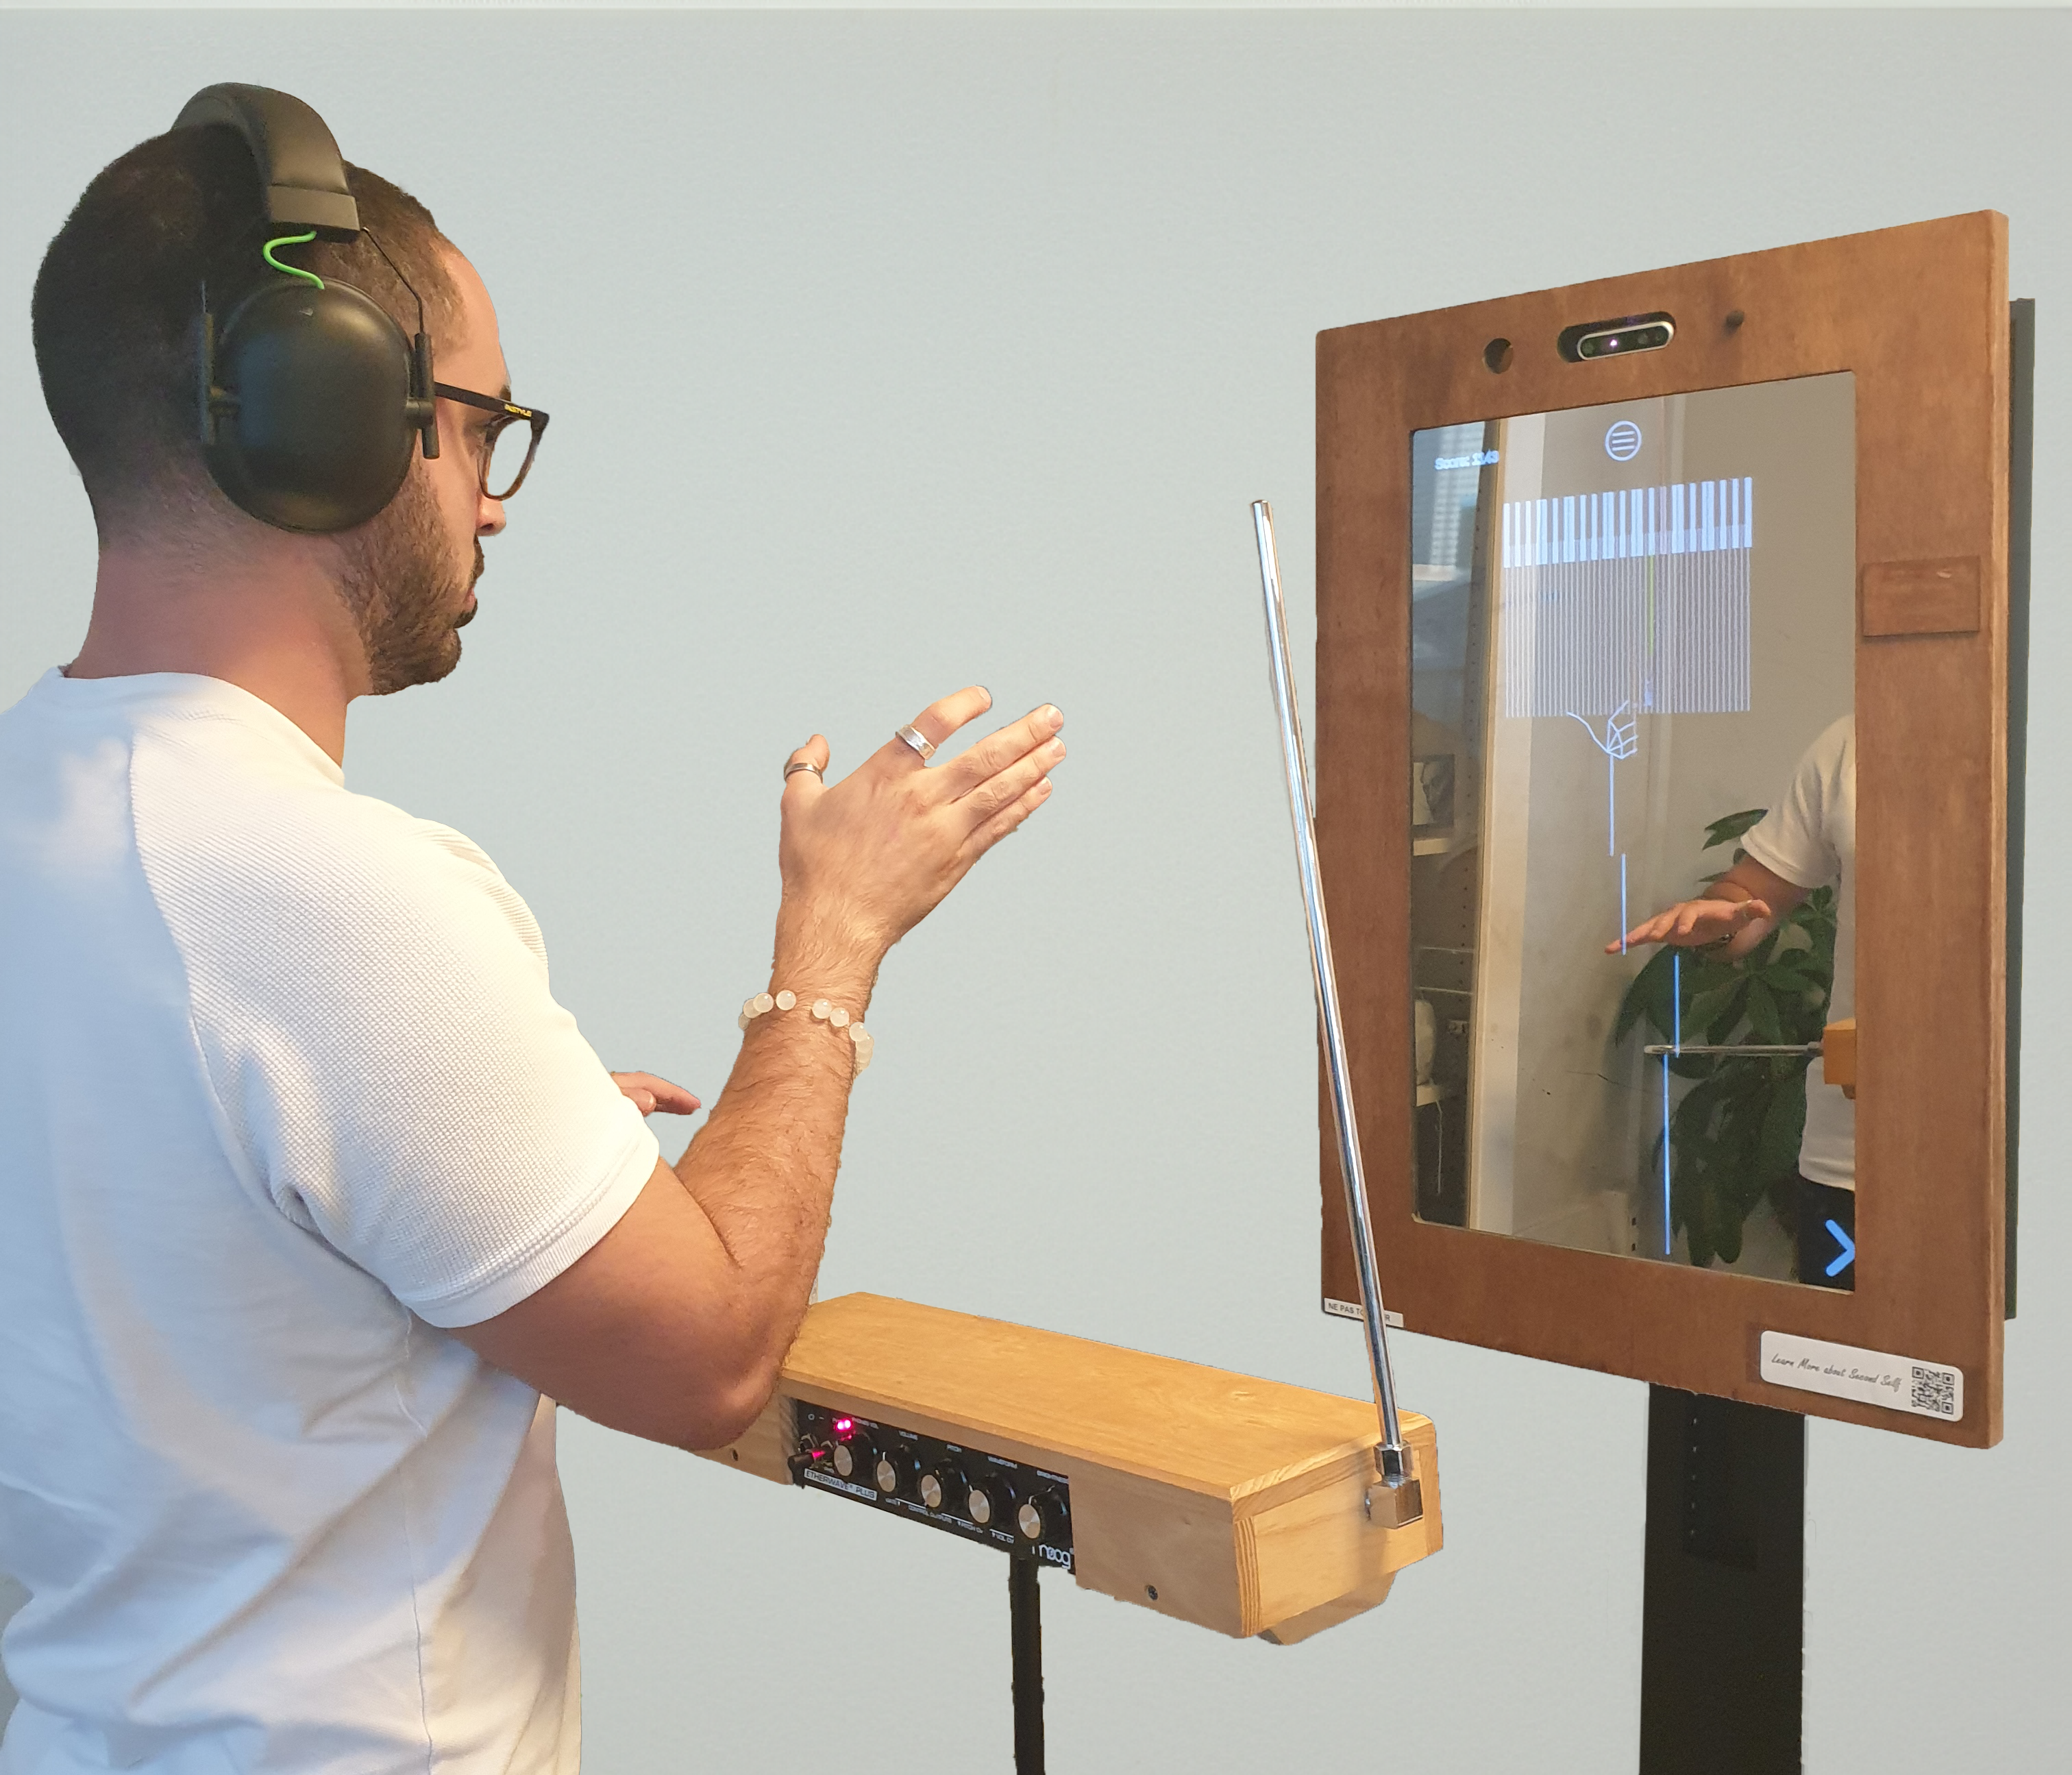
\includegraphics[width=2.2\columnwidth]{AdrLfv_master_thesis/images/polpi_theremine.png}
    \caption{A user testing the theremine learning application.}
    \label{fig:polpi_theremine}
\end{figure}

The user can control a virtual theremin on the mirror, their right hand controlling the pitch horizontally and their left hand the volume vertically. Raising the left hand raises the volume, and lowering it decreases it. Similarly, moving the right hand to the right increases the pitch, and moving it to the left decreases it. 
To launch a note tutorial, people can choose different "scores" in the submenu. When choosing one of them, colored "lines" representing notes come down from the top of the screen.
The user must then position their right hand in space so that the point representing the position of their hand corresponds to the position of the colored line. When the dot is aligned with the color line, the line turns green. The user must hold their hand in this position until the color line disappears. When the color line disappears, the user must reposition it on the following line. When the user successfully aligns the point on their right hand with a colored line, their score increases \ref{fig:theremine_demo}.

\begin{figure}[h]
    \centering
    \includegraphics[width=2.2\columnwidth]{AdrLfv_master_thesis/images/theremine_demo.png}
    \caption{The interface of theremine training application.}
    \label{fig:theremine_demo}
\end{figure}

The point representing the right hand constantly emits particles. These move with acceleration and velocity to mimic an attraction to the ground. Their volume increases and the lines color change when the right hand point is correctly positioned on the falling line. The line turns red when green or red if the user's hand is in the correct or incorrect position.

The screen displays a piano keyboard and white lines indicating its continuity. It allows the user to place his right hand at the desired height. The user can also hide the keyboard and guide bars using a button in the submenu.

\subsection{General Architecture}

The theremine practise module functions similarly to the singing module. The structure is a JavaScript application using the P5 library. The application uses the GOSAI pose estimation driver, subscribing to events providing left and right-hand points provided by Mediapipe.

The program calculated the hand movement values in space one meter from the mirror to match a user's real spatial hand movement values using an actual theremin. For example, moving an note or volume gap with the app means making the same movements as with a theremin. The program maps a real to virtual space regarding notes F2 to B5 (notes before and after this range are not playable). The mirror calculates and displays a projection of two points of the hands on the mirror following the position of the user's hands.

The application calculates the exact positions of the two points from the highest point of the left hand and the rightmost point of the right hand.

\subsection*{User Tests}

The user tests in this project aim to assess a user’s facilitation of learning to play the theremin with the mirror compared to other conventional tools.

\paragraph{Evaluation of the user learning}

\begin{marginfigure}
    \centering
    \includegraphics{AdrLfv_master_thesis/images/carolina_eyck_lver.png}
    \caption{Carolina Eyck playing "La vie en rose" with a theremine.}
    \label{fig:carolina_eyck_thermeine}
\end{marginfigure}

The tests are carried out on 4 people who try to play the theremin without support, and 4 others who try with the notes tutorial on the mirror as support.
The basics of theremin operation are explained to each user. They can test it as much as they like beforehand. We give them tips and techniques to help them play correctly. We show and listen to the first few seconds of "La vie en rose - Carolina Eyck - theremin" (see figure \ref{fig:carolina_eyck_thermeine}).
The subject is asked to try to play on the theremin exactly what he or she has just heard, with the right frequencies. 
The entire sequence of the user study is explained to the user beforehand.

\paragraph[]{Conduct of the tests without the program}
Four users take turns. Each has six tries and can listen to the music in between. The last performance is recorded by capturing the mirror screen. We don't take rhythm into account, but concentrate on the precision of note deviations. We therefore evaluate the user's ability to play valid note deviations without visual support. An audio recording of the performance is made for later evaluation.

\paragraph[]{Conduct of the tests with the program}
Four other users take turns. Each user plays the theremin in front of the program, with the note tutorial correctly calibrated. We record his last performance by capturing a video of the mirror screen. We don't take rhythm into account, concentrating instead on the accuracy of note deviations.

We then carry out an \hyperref[sec:eval_user_exp]{evaluation of the user experience} similar to that of the singing learning application.

\subsection{Results}

\paragraph{Test without program}
The total error is calculated by comparing the frequency difference between each note played and the previous one. We compare each gap between the notes played to the expected intervals in the essential pieces. We consider previous offset errors, i.e., the user may have shifted the frequency by making errors. The sum of all missing or excess semitones in each interval played gives the total error.

We evaluate five people with several training sessions limited to 6 trials. We retrieved the results of the last test. We get an average of 45 semitones offset and many unplayed notes. That is an average of 2.25 semitones of shift per interval. There were many overall frequency shifts in the song (shifts not subsequently corrected).

\paragraph{Test with program}
We calculate the total error by counting the offset in semitones between each note played by the user and the program's objective note. The sum of all offsets gives the total error.
After three trials using the program's tutorial with the theremin, we measured an average offset of 19.66 semitones on the fourth trial. That's an average of 0.98 semitones difference for each note.
Those tested using the program rated their level of fun, giving an average of 5.33/10 after being asked about their experience using it. They gave an average score of 9.33/10 to the understanding of what needs to be done, a score of 5.66/10 to the fluidity of calculations and display, a score of 8/10 to the practicality of the interface and display, and a score of 9.33/10 for the relevance of the tutorial method with the falling scores.

\subsection{Discussion}
We note that the control group (without the program) made approximately twice as many errors as the group using the program despite twice as much training. The program also allows you to avoid global frequency shifts of the songs. We observed a clear progression in user performance ed during the tests. Using the application allows you to learn to play the theremin more quickly and gives a much better visualization of the notes played. The application also allows you to understand better the errors made and correct them more easily.

The most critical problem with this method is the very high accuracy of the theremin, even though the pitch was set to a minimum. It is challenging to play precise notes with the theremin used. The gap between each note is small, the keyboard displayed is very tight, and it isn't easy to place your hand correctly. Lack of precision harms the quality of learning. The use of tutorials from a notes tutorial with augmented reality was considered relevant and effective.

\subsection{Future work}

An interesting capability of the Theremin practice aid app is its ability to turn off its sound to let users practice their theremin in front of the mirror. The application detects the position of the user's hands at the same time as the user plays their instrument. This feature allows him to visualize the note intervals much better, so he can move his hands and position himself more precisely. 

A typical theremin (such as the Moog Music Etherwave Standard used in this project) has a dial for adjusting the accuracy of the detected pitch. This setting set to a minimum allows one to play precise notes, but the difference in physical distance between two notes remains small. Therefore, the keyboard displayed on the screen must be perfectly adapted to match the distance between the notes. Several parameters must be taken into account, such as the mirror/theremin distance, the pitch detection accuracy of the theremin, and the hand detection ability of the mirror camera being slightly tilted downwards. 
A missing feature of the project is the possibility of configuring the size of the displayed keyboard to perfectly adapt to the actual dimensions of the range of notes playable by the theremin according to its placement. We can think about an automatic calibration using the GOSAI frequency estimation and the pose estimation drivers. The application would automatically shift the keyboard displayed on launch, so that the frequency measured by the microphone is the same as the one associated with the user's hand placement.

\section{Conclusion}

This innovative method not only caters to visual learners by providing a dynamic and interactive representation of musical notes, but it also fosters a more intuitive understanding of pitch and timing. The falling notes simulate the real-time progression of a musical piece, allowing learners to synchronize their vocal and musical performance with the visual cues. 
This visual feedback not only enhances the comprehension of musical nuances but also accelerates the learning curve by reinforcing the connection between auditory perception and vocal execution. Moreover, the program's adaptability to different musical genres and the ability to customize difficulty levels make it an inclusive and personalized tool for learners of various skill levels. As technology converges with the art of singing and practising music in general, the incorporation of falling notes tutorials emerges as a promising avenue for more engaging, efficient, and tailored vocal education.